% !TEX TS-program = xelatex
\documentclass[11pt]{article}
\usepackage{lindrew}
\usepackage{xcolor}
\usepackage{amsmath}
\usepackage{amssymb}
\usepackage{amsthm}
\usepackage{fontspec}
\usepackage{bookmark}
\usepackage{tikz}

\title{Math 4547: Real Analysis I}
\author{Lecturer: \textbf{Professor Alex Margolis}\\Notes by: Farhan Sadeek}
\date{Spring 2025}
\begin{document}
\maketitle
\section{January 6, 2025}
Professor Margolis introduced the course and discussed the syllabus. The course
will cover the following topics: Here are some common number systems
\subsection{What is Analysis?}
Analysis is the branch of mathematics that deals with the rigorous study of
limits, functions, derivatives, integrals, and infinite series. It provides the
foundation for calculus and extends its concepts to more abstract settings.

\begin{theorem}
    Every convergent squence is bounded.
\end{theorem}
\subsection{The Real Numbers}
\subsubsection{What are the reals?}

\begin{itemize}
    \item The \vocab{natural Numbers $\mathbb{N}$} = \{1, 2, 3, \ldots\}
    \item The \vocab{integers $\mathbb{Z}$} = \{0, 1, -1, 2, -2, $\cdots$ \}
    \item The \vocab{rational Numbers $\mathbb{Q}$} = \{$\frac{p}{q}$ | $p,q \in
              \mathbb{Z}$ and $q \neq 0$\}
    \item The \vocab{real Numbers $\mathbb{R}$}
    \item The \vocab{complex Numbers $\mathbb{C}$}: = \{ $a + bi$ | $a,b \in
              \mathbb{R}$\}, where $i^2 = -1$
\end{itemize}

\begin{theorem}
    There is no rational number $x$, such that $x^2 = 2$.
\end{theorem}

\begin{proof}
    We assume for contradiction that such an $x$ exists. Then $x = \frac{p}{q}$ for some $p, q \in \mathbb{Z}$ and $q \neq 0$. We can assume that $p$ and $q$ have no common factors. Then, $\frac{p^2}{q^2} = 2$, which implies \[p^2 = 2q^2\] Thus, $p^2$ is even. As the square of an odd number is odd, it follows $p$ must
    even. Therefore, $p = 2k$ for an integer $k$. We have $2q^2 = p^2 = {(2k)}^2 =
        4k^2$, and so $q^2 = 2k^2$. Thus, $q^2$ is even. Since $p$ and $q$ are both
    even, this contradicts our assumption that $p$ and $q$ have no common factors.
    Therefore, there is no rational number $x$ such that $x^2 = 2$.
\end{proof}

This theorem implies, if we visualize $\mathbb{Q}$ as points lying on a number
line, there is a `hole' where $\sqrt{2}$ is. (There are many more `holes' e.g.
$\pi$, $e$, $\sqrt{3}$, \ldots)

The key property that $\mathbb{R}$ possesses, but $\mathbb{Q}$ doesn't is that
$\mathbb{R}$ has ``no holes'' (formally, $\mathbb{R}$ is complete.)

In this class, we will rigorously deduce all properties of $\mathbb{R}$ from
the axioms of the real numbers.

The axioms are in three groups.

\begin{enumerate}
    \item Field Axioms (addition and multiplication)
    \item Order axioms (needed to describe properties concerning inequalities)
    \item Completeness Axiom
\end{enumerate}

\subsection{Addition axioms}
\begin{enumerate}
    \item For every pair $a, b \in \mathbb{R}$, we can associate a real number $a + b$
          called their \vocab{sum}.
    \item For every real number $a$, there is a real number $-a$ called its
          \vocab{negative} or \vocab{additive inverse}.
    \item There is a special real number $0$ called zero or the additive identity such
          that for all $a, b, c, x, y, z \cdots $ are real numbers unless otherwise
          stated:
          \begin{enumerate}
              \item $a + b = b + a$
              \item $a + (b + c) = (a + b) + c$
              \item $a + 0 = a$
              \item $a + (-a) = 0$
          \end{enumerate}
\end{enumerate}

\section{January 8, 2025}
In this lecture, we will use the axioms to deduce various properties of the
real numbers $\mathbb{R}$. From these axioms, we can derive many more
properties of the real numbers.

\begin{proposition}
    If $x + a = x$ for all $a \in \mathbb{R}$, then $a = 0$.
\end{proposition}

\begin{proof}
    We know that
    \begin{equation*}
        \begin{aligned}
            x & = x + 0 \quad \text{(A3)}                   \\
              & = x + a \quad \text{(by assumption on $a$)}
        \end{aligned}
    \end{equation*}
    By the left cancellation property of addition, it follows that $a = 0$.
\end{proof}

\begin{proposition}[Left cancellation of addition]
    If $a + x = a + y$, then $x = y$.
\end{proposition}

\begin{proof}
    We start with the given equation $a + x = a + y$. By the additive identity property (A3), we have:
    \begin{align*}
        y & = y + 0          & \text{(A3)}    \\
          & = y + (a + (-a)) & \text{(A4)}    \\
          & = (y + a) + (-a) & \text{(A2)}    \\
          & = (a + y) + (-a) & \text{(A1)}    \\
          & = (a + x) + (-a) & \text{(given)} \\
          & = x + (a + (-a)) & \text{(A1)}    \\
          & = x + 0          & \text{(A4)}    \\
          & = x              & \text{(A3)}
    \end{align*}
    Therefore, $x = y$.
\end{proof}

\begin{proposition}
    $-(-a) = a$
\end{proposition}

\begin{proof}
    We need to show that $-(-a) = a$. Consider the following:
    \begin{align*}
        (-a) + (-(-a)) & = 0 \quad \text{(by definition of additive inverse)} \\
        (-a) + a       & = 0 \quad \text{(since } -(-a) = a)                  \\
        a + (-a)       & = 0 \quad \text{(by commutativity of addition)}      \\
        (-a) + (-(-a)) & = a + (-a) \quad \text{(by substitution)}            \\
        (-(-a))        & = a \quad \text{(by left cancellation of addition)}
    \end{align*}
    Therefore, $-(-a) = a$.
\end{proof}

\begin{proposition}
    $-(a + b) = (-a) + (-b)$
\end{proposition}

\begin{proof}
    We need to show that the additive inverse of $(a + b)$ is equal to the sum of the additive inverses of $a$ and $b$. Consider the following:
    \begin{align*}
        (a + b) + (-(a + b))    & = 0 \quad \text{(by definition of additive inverse)}                  \\
        (a + b) + ((-a) + (-b)) & = a + (b + ((-a) + (-b))) \quad \text{(by associativity of addition)} \\
                                & = a + ((b + (-a)) + (-b)) \quad \text{(by associativity of addition)} \\
                                & = a + ((-a) + (b + (-b))) \quad \text{(by commutativity of addition)} \\
                                & = a + ((-a) + 0) \quad \text{(by definition of additive inverse)}     \\
                                & = a + (-a) \quad \text{(by identity property of addition)}            \\
                                & = 0 \quad \text{(by definition of additive inverse)}
    \end{align*}
    Therefore, $-(a + b) = (-a) + (-b)$.
\end{proof}

\begin{proposition}
    $-0 = 0$
\end{proposition}

\begin{proof}
    We need to show that the additive inverse of $0$ is $0$. Consider the following:
    \begin{align*}
        0 + 0    & = 0 \quad \text{(by the identity property of addition, A3)}  \\
        0 + (-0) & = 0 \quad \text{(by the definition of additive inverse, A4)}
    \end{align*}
    Therefore, we have:
    \begin{align*}
        0 + 0 & = 0 + (-0)
    \end{align*}
    By the left cancellation property of addition, it follows that:
    \begin{align*}
        0 & = -0
    \end{align*}
    Therefore, $-0 = 0$.
\end{proof}

\subsection{Multiplication Axioms}

\begin{definition}
    For all $a, b \in \mathbb{R}$, we can associate a real number $a \times b$ called their \vocab{product}.
\end{definition}

\begin{definition}
    For every $a \in \mathbb{R}$, there is some $a^{-1} \in \mathbb{R}$ called its \vocab{multiplicative inverse} or \vocab{reciprocal} such that for all $a \neq 0$, $a \times a^{-1} = 1$.
\end{definition}

\begin{definition}
    There is a number 1 called \vocab{one} or the \vocab{multiplicative identity} such that for all $a \in \mathbb{R}$, $a \times 1 = a$.
\end{definition}

\begin{definition}
    For all $a, b, c \in \mathbb{R}$, we have the following properties of multiplication:
    \begin{itemize}
        \item For all $a, b \in \mathbb{R}$, $a \times b = b \times a$.
        \item For all $a, b, c \in \mathbb{R}$, $a \times (b \times c) = (a \times b) \times
                  c$.
        \item For all $a \in \mathbb{R}$, $a \times 0 = 0$.
        \item For all $a, b \in \mathbb{R}$, $a \times (b + c) = a \times b + a \times c$.
    \end{itemize}
\end{definition}

\begin{proposition}
    If $a \times b = a$, and $a \in \mathbb{R}$ then $b = 1$.
\end{proposition}

\begin{proof}
    We start with the given equation $a \times b = a$. By the multiplicative identity property, we have:
    \begin{align*}
        a \times b & = a \times 1                                              \\
        b          & = 1 \quad \text{(by left cancellation of multiplication)}
    \end{align*}
    Therefore, $b = 1$.
\end{proof}

\begin{proposition}
    If $a \neq 0$ and $a \times b = a \times c$, then $b = c$.
\end{proposition}

\begin{proof}
    We start with the given equation $a \times b = a \times c$. By the multiplicative inverse property, we have:
    \begin{align*}
        a^{-1} \times (a \times b) & = a^{-1} \times (a \times c) \\
        (a^{-1} \times a) \times b & = (a^{-1} \times a) \times c \\
        1 \times b                 & = 1 \times c                 \\
        b                          & = c
    \end{align*}
    Therefore, $b = c$.
\end{proof}

\begin{proposition}
    If $a \neq 0$ and $a^{-1} \neq 0$, then $(a^{-1})^{-1} = a$.
\end{proposition}

\begin{proof}
    We need to show that the multiplicative inverse of $a^{-1}$ is $a$. Consider the following:
    \begin{align*}
        a^{-1} \times a             & = 1 \quad \text{(by definition of multiplicative inverse)} \\
        (a^{-1})^{-1} \times a^{-1} & = 1 \quad \text{(by definition of multiplicative inverse)} \\
        (a^{-1})^{-1}               & = a
    \end{align*}
    Therefore, $(a^{-1})^{-1} = a$.
\end{proof}

\begin{proposition}
    If $a \neq 0$, $b \neq 0$, and $a \times b \neq 0$, then $(a \times b)^{-1} = a^{-1} \times b^{-1}$.
\end{proposition}

\begin{proof}
    We need to show that the multiplicative inverse of $a \times b$ is $a^{-1} \times b^{-1}$. Consider the following:
    \begin{align*}
        (a \times b) \times (a^{-1} \times b^{-1}) & = a \times (b \times (a^{-1} \times b^{-1})) \\
                                                   & = a \times ((b \times a^{-1}) \times b^{-1}) \\
                                                   & = a \times (1 \times b^{-1})                 \\
                                                   & = a \times b^{-1}                            \\
                                                   & = 1
    \end{align*}
    Therefore, $(a \times b)^{-1} = a^{-1} \times b^{-1}$.
\end{proof}

\begin{proposition}
    If $a, b, c \in \mathbb{R}$, then $(a + b) \times c = (a \times c) + (b \times c)$.
\end{proposition}

\begin{proof}
    We need to show that the product of $(a + b)$ and $c$ is equal to the sum of the products of $a$ and $c$, and $b$ and $c$. Consider the following:
    \begin{align*}
        (a + b) \times c & = c \times (a + b)        \\
                         & = c \times a + c \times b \\
                         & = a \times c + b \times c
    \end{align*}
    Therefore, $(a + b) \times c = (a \times c) + (b \times c)$.
\end{proof}

\begin{proposition}
    For all $a \in \mathbb{R}$, $a \times 0 = 0$.
\end{proposition}

\begin{proof}
    We need to show that the product of any real number $a$ and $0$ is $0$. Consider the following:
    \begin{align*}
        a \times 0 & = a \times (0 + 0)        \\
                   & = a \times 0 + a \times 0 \\
                   & = 0 + 0                   \\
                   & = 0
    \end{align*}
    Therefore, $a \times 0 = 0$.
\end{proof}

\begin{proposition}
    If $a \times b = 0$, then either $a = 0$ or $b = 0$ or both.
\end{proposition}

\begin{proof}
    We need to show that if the product of $a$ and $b$ is $0$, then either $a$ or $b$ or both must be $0$. Consider the following:
    \begin{align*}
        a \times b = 0
    \end{align*}
    If $a \neq 0$, then $b = 0$ by the multiplicative inverse property. If $b \neq 0$, then $a = 0$ by the multiplicative inverse property. Therefore, if $a \times b = 0$, then either $a = 0$ or $b = 0$ or both.
\end{proof}

\begin{proposition}
    $a \times (-b) = (-a) \times b$. In particular, $a \times (-1) = -a$.
\end{proposition}

\begin{proof}
    We need to show that the product of $a$ and $-b$ is equal to the product of $-a$ and $b$. Consider the following:
    \begin{align*}
        a \times (-b) + a \times b & = a \times (b + (-b))          \\
                                   & = a \times 0                   \\
                                   & = 0                            \\
                                   & = a \times b + (-(a \times b))
    \end{align*}
    Hence, the additive inverse of $a \times b$ is $-(a \times b)$. Therefore, $a \times (-b) = (-a) \times b$.
\end{proof}

\begin{proposition}
    $(-1) \times (-1) = 1$
\end{proposition}

\begin{proof}
    We need to show that the product of $-1$ and $-1$ is $1$. Consider the following:
    \begin{align*}
        (-1) \times (-1) & = -(-1) \times 1          \\
                         & = -(-1) \times (1 + 0)    \\
                         & = -(-1) \times (1 + (-1)) \\
                         & = -(-1) \times 0          \\
                         & = 0                       \\
                         & = (-1) + (-1)
    \end{align*}
    Therefore, $(-1) \times (-1) = 1$.
\end{proof}

\section{January 10, 2025}

For all \(a, b \in \mathbb{R}\), we write:
\begin{itemize}
    \item \(ab\) or \(a \cdot b\) for \(a \times b\).
    \item \(a - b\) for \(a + (-b)\).
    \item \(\frac{1}{a}\) for \(a^{-1}\) if \(a \neq 0\).
    \item \(\frac{a}{b}\) for \(a b^{-1}\) if \(b \neq 0\).
\end{itemize}
For \(a \neq 0\), we write:
\begin{itemize}
    \item \(a^0\) for 1.
    \item \(a^{k + 1}\) for \(a^k \cdot a\) for \(k = 0, 1, 2, \ldots\)
    \item \(a^{-1} for (a^l)^{-1}\) for \(l = 1, 2, 3\)
\end{itemize}

\begin{definition}
    Any set equipped with operations \(+\) and \(\times\) staisfying A1 - A4, M1 - M4, Z, D is a \vocab{field}.
\end{definition}
\begin{fact}
    Some facts about the fields:

    \begin{itemize}
        \item \(\RR, \QQ, \CC\) are all fields.
        \item \(\ZZ\) is not a field (M4 isn't satisified).
        \item \(\NN\) is not a field (\(A4, M4\)) are not satsified.
        \item \(\frac{\ZZ}{p\ZZ}\) (integers mod p for prime \(p\)) is a field.
    \end{itemize}
\end{fact}

\subsection{The order axioms}
The order axioms are: There is as subset of \(P \subset \RR\) called the set of
\textbf{positive numbers}.
\begin{itemize}
    \item If \(a, b \in \PP\), then \(a + b \in \PP\). \hfill (P1)
    \item If \(a, b \in \PP\), then \(a \times b \in \PP\). \hfill (P2)
    \item For each \(a \in \RR\), exactly one of the following is true: \(a \in \PP\),
          \(a = 0\), or \(-a \in \PP\). \(\leftarrow\) \text{Law of Trichotomy}\hfill
          (P3)
\end{itemize}
\textbf{P3} is the most powerful aximom about the positive numbers.
\begin{proposition}
    Prove that \(1 \in \PP\)
\end{proposition}
\begin{proof}
    According to \textbf{P3}, either
    \begin{itemize}
        \item \(1 \in \PP\)
        \item \(1 = 0\)
        \item \(-1 \in \PP\)
    \end{itemize}
    We will prove (b) and (c) are false by contradiction and then show that \(1 \in \PP\).
    If \textbf{(b)} holds, \(1 = 0\), which contradicts \textbf{Z}.
    Assume for contradiction \textbf{(c)} holds. We know from last lecture that \(1 = -(-1)\). Since \(-1 \in \PP\), by (P2), \((-1) \times (-1) \in \PP\). But \((-1) \times (-1) = 1\), so \(1 \in \PP\).
    \(\therefore, 1 \in \PP\) and \(-1 \in \PP\) contradicts \textbf{P3}.
    Since, \textbf{(b)} and \textbf{(c)} cannot hold, therefore, \textbf{(a)} must hold.
\end{proof}

\begin{fact}
    For all \(a , b \in \RR\), we write
    \begin{itemize}
        \item \(a < b\) if \(b - a \in \PP\)
        \item \(a > b\) if \(a - b \in \PP\)
        \item \(a \leq b\) if \(b - a \in \PP \cup \{0\}\)
        \item \(a \geq b\) if \(a - b \in \PP \cup \{0\}\)
    \end{itemize}
\end{fact}

\begin{proposition}
    \(a > b\) if and only if \(-a < -b\). In particular, \(x > 0 \Longleftrightarrow -x < 0\)
\end{proposition}
\begin{proof}
    \begin{align*}
        a > b & \Longleftrightarrow  a - b \in \PP        \\
              & \Longleftrightarrow  -(-(a)) - b \in -\PP \\
              & \Longleftrightarrow  -b -(-a) \in -\PP    \\
              & \Longleftrightarrow  -a < -b
    \end{align*}
\end{proof}
\begin{proposition}
    For all \(x, y, z \in \RR\) the following holds:
    \begin{itemize}
        \item \(x \leq x\)
        \item If \(x \leq y\) and \(y \leq z\), then \(x \leq z\).
        \item If \(x \leq y\) and \(y \leq z\), then \(x \leq z\).
    \end{itemize}
\end{proposition}
\begin{proof}

\end{proof}

\begin{proposition}
    If \(x, t, z \in \RR\) and \(x < y\), then \(x + z < y + z\).
\end{proposition}
\begin{proof}
    Since \(x < y\), we have \(x - y \in \PP\).
    By the properties of addition (A1-A4), we know that:
    \[
        (y + z) - (x + z) = y - x
    \]
    Since \(y - x \in \PP\), it follows that:
    \[
        (y + z) - (x + z) \in \PP
    \]
    Hence, \(x + z < y + z\).
\end{proof}

\begin{proposition}
    If \(x, y, z \in \RR\) and \(x < y\) and \(z > 0\), then \(xz < yz\).
\end{proposition}

\begin{proof}
    \(zy = zx = z(y - x) \). Now, \(z \in \PP\) and \(y - x \in \PP\), therefore \(zy - zx \in \PP\). Therefore, \(xz < yz\).
\end{proof}
\begin{corollary}
    If \(x, y, z \in \RR\) and \(x < y\) and \(z < 0\), then \(xz > yz\).
\end{corollary}
\begin{proof}

\end{proof}
\begin{corollary}
    For all, \(a \in \RR\), \(a^2 \geq 0\).
\end{corollary}
\begin{proof}
    By P3, either \(a > 0, a = 0\) or \(g < 0\).
    \begin{itemize}
        \item If \(a > 0\), then \(a^2 = a \times a > 0\). \hfill(P2)
        \item If \(a = 0\), then \(a^2 = 0 \geq 0\).
        \item If \(a < 0\), then \(-a > 0\) and \((-a)^2 = a^2 > 0\).
    \end{itemize}
\end{proof}

\begin{proposition}
    If \(x \in \PP\), then \(x^{-1} \in \PP \).
\end{proposition}
\begin{proof}
    Since, \(x \in \PP, x \neq 0\). Therefore, \(x^{-1}\) exists. By P3, \(x^{-1} > 0, x^{-1} = 0  \), or \(x^{-1} < 0\).
    If \(x^{-1} = 0\), then \(1 = x \times x^{-1} = x \times 0 = 0\)
    [Contradiction] Assume \(x^{-1} < 0\). Then \(-x^{-1} \in \PP\) by P3. Then \(x
    \times (-x^{-1}) \in \PP\) by P2. But \(x \times (-x^{-1}) = -1\), which
    contradicts P3 since \(-1 \notin \PP\). Therefore, \(x^{-1} \in \PP\).
\end{proof}
\begin{corollary}
    If \(x, y \in \PP\), and \(x < y\), then \(\frac{1}{y} < \frac{1}{x}\).
\end{corollary}

\section{January 13, 2025}
Homework 1 is due on January 21, 2025.\\
\begin{definition}
    We define \(\max \colon \RR \times \RR \Rightarrow \RR\) by \[\max(a, b) = \begin{cases}
            a & \text{if } a \geq b \\
            b & \text{if } b \geq a
        \end{cases}\]
\end{definition}

\begin{definition}
    We define \(\max \colon \RR \times \RR \to \RR\) by \[\max(a, b) = \begin{cases}
            a & \text{if } a \geq b \\
            b & \text{if } b > a
        \end{cases}\]
\end{definition}
\begin{definition}
    We define \(|x|\) \(\colon \RR \rightarrow \RR\) as follows:
    \[
        |x| = \begin{cases}
            x  & \text{if } x \geq 0 \\
            -x & \text{if } x < 0
        \end{cases}
    \]
\end{definition}
\begin{proposition}
    For all \(x \in \RR\), \(|-x| =  |x|\).
\end{proposition}
\begin{proof}
    By P3, x > 0, x = 0, or x < 0. \\
    \begin{itemize}
        \item Case 1: If \(x > 0\), then \(|x| = x\) and \(|-x| = -(-x) = x\). Thus, \(|x| =
              |-x|\).
        \item Case 2: If \(x = 0\), then \(|x| = 0\) and \(|-x| = -0 = 0\). Thus, \(|x| =
              |-x|\).
        \item Case 3: If \(x < 0\), then \(|x| = -x\) and \(|-x| = -(-x) = x\). Thus, \(|x| =
              |-x|\).
    \end{itemize}
\end{proof}

\begin{theorem} [The Triangle \(\Delta\) Inequality]
    For all \(a, b, \in \RR\) \[ |a + b| = \leq |a| + |b| \] with equality if and only if either \( a \geq 0\) and \( b \geq 0\) or \(a \leq
    0\) and \(b \leq 0\).
\end{theorem}

\begin{proof}
    By P3, oen of the following 8 Cases must hold: \\
    \begin{center}

        \begin{tabular}{|c|c|c|c|}
            \hline
              & a          & b            & a + b        \\ \hline
            1 & \(\geq\) 0 & \(\geq\) 0   & Row 2, Col 4 \\ \hline
            2 & \(\geq\) 0 & \(\geq\) 0   & Row 3, Col 4 \\ \hline
            3 & \(\geq\) 0 & \( < \) 0    & Row 4, Col 4 \\ \hline
            4 & \(\geq\) 0 & \( < \) 0    & Row 5, Col 4 \\ \hline
            5 & \(< \) 0   & Row 6, Col 3 & Row 6, Col 4 \\ \hline
            6 & \(< \) 0   & Row 7, Col 3 & Row 7, Col 4 \\ \hline
            7 & \(< \) 0   & Row 8, Col 3 & Row 8, Col 4 \\ \hline
            8 & \(< \) 0   & Row 8, Col 3 & Row 8, Col 4 \\ \hline
        \end{tabular}
    \end{center}
    Case 2 and 7 is not possible. But we will prove the rest of the cases:
    \begin{itemize}
        \item[(1)] \(|a| = a\), \(|b| = b\), \(|a + b| = a + b\), $\therefore$ \(|a + b| = a + b = |a| + b\)
        \item [(3)]
        \item [(4)] \(|a| = a, |b| = -b, |a + b| = a + b\)
              \begin{align*}
                  |a + b| = - a- b = - 0 - b & = (-a \leq 0)                           \\
                                             & \leq a + 0 \quad \text{(since $b < 0$)} \\
                                             & = |a| + |b|
              \end{align*}
        \item [(5)] Follows the similarly by symmetry.

    \end{itemize}
    Finish this for exercise.
\end{proof}
The picture of the Triangle identity
\begin{center}

    \begin{tikzpicture}
        \coordinate [label=left:A] (A) at (0,0);
        \coordinate [label=right:B] (B) at (4,0);
        \coordinate [label=above:C] (C) at (2,3);

        \draw (A) -- node[below] {$c$} (B);
        \draw (B) -- node[right] {$a$} (C);
        \draw (C) -- node[left] {$b$} (A);
    \end{tikzpicture}
\end{center}
\[ |a| = ||\vec{BC}|| \leq |b| + |c| = ||\vec{AC}|| + ||\vec{AB}|| \]
\begin{proposition}
    For all \(a, b, \in \RR\) \[ |ab| = |a|\cdot|b|\]
\end{proposition}
\begin{proof}
    If \(a = 0\) or \(b = 0\), then \(|ab| = |0| = 0 = |a|\cdot|b|\)
    Let's assume that \(a \neq 0, b \neq 0\).
    \begin{itemize}
        \item \(a > 0, b > 0\) Then P2 implies \(ab > 0\) so, \(|ab| = ab = |a||b|\)
        \item \(a < 0, b > 0\). Then \(ab < 0\). Then \(|ab| = -ab = (-a)b = |a||b|\)
        \item \(a > 0, b < 0\). This follows from case 2 by symmetry.
        \item \(a < 0, b < 0\).Then \(ab > 0\). Hence, \(|ab| = ab = (-a)(-b) = |a||b|\)
    \end{itemize}
\end{proof}

\begin{theorem} [Bernouli's Inequality]
    For all \(x \in \RR\) with \(x > -1\) and \(n \in \NN\), if \(n \geq 1\), then \[(1 + x)^n \geq 1 + nx\]
\end{theorem}
\begin{proof}
    We proceed by induction on \(n\). \\
    Base Case: \(n = 1\) \(\colon (1 + x)^{1} = 1 + x = 1 + 1 \cdot x\)\\
    Inductive Step: Assume
    \[
        (1 + x)^N \geq 1 + Nx
    \]
    We want to show \((1 + x)^{N + 1} \geq 1 + (N + 1) \cdot x\). First, since \(x
    > -1\), \(x + 1 > 0\). \\ Multiplying both sides by \(x + 1\),
    \begin{align*}
        (1 + x)(1 + x)^N & \geq (1 + Nx)(1 + x)                                          \\
                         & = 1 + (N + 1)x + Nx^2 \quad \text{(field axioms)}             \\
                         & \geq 1 + (N + 1)x \quad \text{(since \(N > 0\), \(x^2 > 0\))}
    \end{align*}
    Hence, \((1 + x)^{N + 1} \geq 1 + (N + 1)x\).
\end{proof}
\section{January 15, 2025}
\subsection{The completeness axiom}
Let \(B \subseteq \RR\). We say the following:
\begin{itemize}
    \item We say \(b_1 \subseteq\) is a \underline{least element} or \underline{minimum}
          of \(B\) if
          \begin{itemize}
              \item \(b_1 \in B\), and
              \item \(b_1 \leq b\) for all \(b \in B\).
          \end{itemize}
          We write \(b_1 = \min B\).

    \item We say \(b_1 \subseteq\) is a \underline{least element} or \underline{minimum}
          of \(B\) if
          \begin{itemize}
              \item \(b_1 \in B\), and
              \item \(b_1 \leq b\) for all \(b \in B\).
          \end{itemize}
          We write \(b_1 = \min B\).
\end{itemize}
\begin{example}
    Let \(B = \{1, 2, 3\}\). Then \(\min B = 1\) and \(\max B = 3\).
\end{example}

\begin{proposition}
    Let \(B \subseteq R\). The maximum of \(B\) (if it exists) is unique. Let Similarly, the minimum of \(B\) is unique.
\end{proposition}
\begin{proof}
    Suppose \(a, b \in \RR\) are both maximum of \(B\). Since \(a \in B\) and \(b\) is a max of \(B\), \(a ,\leqslant b\). Similarly, \(b \leqslant a\).Since \(a \leqslant b\) and \(b \leqslant a\), \(a = b\)
\end{proof}

\begin{definition}
    Let \(B \subseteq \mathbb{R}\).
    \begin{itemize}
        \item We say \(h\) is a \vocab{lower bound} of \(B\) if \(h \leq b\) for all \(b \in
              B\).
        \item We say \(h\) is an \vocab{upper bound} of \(B\) if \(b \leq h\) for all \(b \in
              B\).
    \end{itemize}
\end{definition}
\begin{example}
    Let \(B = [1, 2)\). Then \(1\) is a lower bound of \(B\) and \(2\) is an upper bound of \(B\). Note that \(1\) is the minimum of \(B\), but \(2\) is not the maximum of \(B\) since \(2 \notin B\).
\end{example}
\begin{definition}
    Let \(B \in \RR\). We say \(B\) is \begin{itemize}
        \item \vocab{bounded above} if there exists an upper bound of \(B\).
        \item \vocab{bounded below} if there exists a lower bound of \(B\).
        \item \vocab{bounded} if there exists an upper bound and a lower bound of \(B\).
    \end{itemize}
\end{definition}
\begin{fact}

\end{fact}
\begin{example}
    \begin{itemize}
        \item \(\NN\) is bounded below, but not bounded above.
        \item \((- \infty, 1]\) is bounded above but not bounded below
        \item \((1, 3)\) is bounded.
    \end{itemize}
\end{example}

\subsection{Completeness Axiom}
\begin{definition}
    A set \(B \subseteq \mathbb{R}\) is said to be \textbf{bounded above} if there exists a real number \(M\) such that \(b \leq M\) for all \(b \in B\). The number \(M\) is called an \textbf{upper bound} of \(B\).
\end{definition}

\begin{definition}
    A real number \(s\) is called the \textbf{supremum} or \textbf{least upper bound} of a set \(B \subseteq \mathbb{R}\) if:
    \begin{enumerate}
        \item \(s\) is an upper bound of \(B\).
        \item If \(u\) is any upper bound of \(B\), then \(s \leq u\).
    \end{enumerate}
    We denote the supremum of \(B\) by \(\sup B\).
\end{definition}

\begin{theorem}[Completeness Axiom]
    Every non-empty set \(B \subseteq \mathbb{R}\) that is bounded above has a supremum.
\end{theorem}

\begin{example}
    \(2 = \sup([1, 2])\)
\end{example}
\begin{proof}
    Suppose, \(t\) is an upper bound of \(B\). Suppose towards a contradiction that \(t < 2\). Then \[1 \leqslant t < \frac{t + 2}{2} < \frac{2 + 2}{2} = 2\]
    So, \(\frac{t + 2}{2}\) is an element of the set \(B\) that is strictly bigger
    than \(t\) but we arrived to a contradictiopn. Therefore, \(2 \leqslant t\).
    Since \(2\) is an upper bound of \(B\) = sup(\(B\)).
\end{proof}

\begin{example}
    The empty set \(\phi \in \RR\) has no supremeum since \(\RR\) is the set of upper bounds of \(\phi\) and \(\RR\) has no leas element.
\end{example}

\begin{proposition}
    If \(B \in \RR\) and \(\max(B)\) exists then \(\max(B) = \sup(B)\).
\end{proposition}

\begin{proof}
    Let \(A = \max(B)\). Then \( B\) is non-empty and bounded is above by \(a\). If \(C = \sup(B)\), then \(a \leq c\). Since \(c\) is an upper bound \(a \in B\). Also \(c \leqslant a\). Since, \(c\) is the least upper bound. \(\therefore a = c\)
\end{proof}

\begin{proposition}[The approximation property of suprema]
    Let \(B \subseteq \RR\) be non-empty and bounded above. For any \(\epsilon > 0\), there exists an element \(b \in B\) such that \(\sup B - \epsilon < b \leq \sup B\).
\end{proposition}
\begin{proof}
    Suppose for contradicton there was some \(\epsilon > 0\) such that no \(b\) as above exists. Then for all \(c \in B, c \leqslant \sup(B) - \epsilon\) i.e. \(\sup(B) - \epsilon\) is an upper bound of \(B\). But \(\sup(B)\) is the least upper bound of \(B\), so \(\sup(B) - \epsilon < \sup(B)\). This is a contradiction. Therefore, there must exist some \(b \in B\) such that \(\sup(B) - \epsilon < b \leq \sup(B)\).
\end{proof}

\begin{remark}
    To prove \(a\) is a supremum of \(B\), we need show the following:
    \begin{itemize}
        \item \(a\) is an upper bound of \(B\).
        \item If \(c\) is an upper bound of \(B\), then \(a \leqslant c\).
    \end{itemize}
\end{remark}

\begin{theorem}
    Suppose, \(F \subseteq \RR\) is non-empty and bounded below. Then, there exist a \vocab{greatest lower bound} of \(\FF\), called \vocab{infimum} of F, denoted \(\inf(F)\).
\end{theorem}
\begin{proof}
    Let \(B = \{x \in \RR \mid -x \in F\}\). We will show:
    \begin{itemize}
        \item \(B\) is bounded above and non-empty, hence \(a = \sup(B)\) exists.
        \item \(-a\) is a lower bound of \(F\).
        \item If \(c\) is a lower bound of \(F\), then \(c \leqslant -a\).
    \end{itemize}
    \begin{itemize}
        \item Since \(F\) is non-empty, \(B\) is non-empty. Suppose \(c\) is a lower bound of
              \(F\). Let \(x \in B\). Then \(-x \in F\), so \(-x \geqslant c \rightarrow x
              \leqslant -c\). Hence, \(c\) is an upper bound of \(B\). Therefore, \(B\) is
              bounded above.
        \item Let \(f \in F\). Then \(-f \in B\), so \(-f \leq a\) (since \(a = \sup(B)\)).
              Therefore, \(f \geq -a\). Hence, \(-a\) is a lower bound of \(F\).
        \item Let \(c\) be a lower bound of \(F\). Let \(b \in B\). Then \(-b \in F\), so
              \(-b \geq c \rightarrow b \leq -c\). Hence, \(-c\) is an upper bound of \(B\).
              Therefore, \(-a \leq -c \rightarrow c \leq -a\).
    \end{itemize}
\end{proof}
\section{January 17, 2025}
\begin{corollary}
    Let \(F\) be a non-empty and bounded below for each \(\epsilon > 0\), there exists \(f \in F\) such that \[ \inf (F) \leqslant f < \inf(F) + \epsilon\]
\end{corollary}

\begin{theorem}
    There is a unique positive number \(\alpha\) such that \(\alpha^2 = 2\).
\end{theorem}

\begin{proof}
    Let \(E = \{x \in \RR \mid x^2 < 2\}\). Since, \(x^1 = 1 < 2\), so \(1 \in E\), so \(E \neq 0\). \\
    Suppose, \(x \geqslant 2\). Then \(x^2 \geqslant 2^2 = 4 > 2\). Hence, \(x \notin E\).
    Therefore, if \(x \in E\), then \(x < 2\). \\
    Hence, \(E \neq 0\), and bounded above by 2. \\
    Let \(\alpha = \sup(E)\). \\
    We know that \(1 \leqslant \alpha \leqslant 2\). \\
    If \(\alpha^2 \neq 2\), then either \(\alpha^2 = 2\), then either \(\alpha^2 > 0\) or \(\alpha^2 < 2\). We'll show that both these cases lead to contradiction!
    \begin{itemize}
        \item[Case 1:] When \(\alpha^2 < 2\) Let \(h = \frac{1}{2} \min(\alpha, \frac{2 -
                \alpha^2}{3\alpha})\). Note \(h > 0, h < \alpha\) and \(h < \frac{2
                -\alpha^2}{3\alpha}\). Note that \((\alpha + h)^2 = \alpha^2 + 2\alpha h + h^2
            < \alpha^2 + 3\alpha h < \alpha^2 + 3\alpha \frac{2 - \alpha^2}{3\alpha} = 2\).
            So \(\alpha + h \in E\). Since \(\alpha + h > \alpha\), this contradicts
            \(\alpha = \sup(E)\).
        \item[Case 2:] When \(\alpha^2 > 2\) We set \(h = \frac{1}{2} \frac{\alpha^2 -
                2}{2\alpha} > 0\). Since \(\alpha - h < \alpha\), the approximation property
            says that there exists \(e \in E\) such that \[\alpha - h < e \leqslant \alpha\]. Then \((\alpha - h)^2 < e^2\). Then \(\alpha^2 - 2\alpha h + h^2 < 2 \Rightarrow \alpha^2 - 2\alpha h < 2\). Therefore, \(h > \frac{\alpha^2 - 2}{2\alpha}\). And we arrived at a contradiction. Since \(\alpha^2 < 2\) and \(\alpha^2 > 2\) cannot hold, so \(\alpha^2 = 2\).
    \end{itemize}
    Suppose \(\alpha^2 = \beta^2 = 2\) and \(\alpha, \beta > 0\). Then \(\alpha^2 - \beta^2 = (\alpha + \beta)(\alpha - \beta) = 0\). Since \(\alpha + \beta > 0, \alpha - \beta = 0 \). Hence, \(\alpha = \beta\)
\end{proof}

\begin{remark}
    The same proof shows \{\(\alpha \in \QQ \mid \alpha^2 = 2\)\} cannot have a supremum in \(\QQ\), i.e.\ completeness doesn't hold.
\end{remark}

% Create a notation thing for this notes
\begin{remark}
    We denote \(\alpha\) as above using \(\sqrt{2}\) by modifying the previous proof.
\end{remark}

\begin{theorem}
    For any positive real number \(x\), there exist unique postitive real number, denoted \(\sqrt{2}\), such that \((\sqrt{x})^2 = x\).
\end{theorem}

\begin{theorem}[Archimedean Property for Real Numbers]
    Let \(x \in \RR\). Then there exists a natural number \(n \in \NN\) such that \(n > x\).
\end{theorem}

\begin{proof}
    Suppose this theorem is not true for some \(x \in \RR\). Then \(x\) is an upper bound of \(\NN\). Since \(\NN \neq 0, \alpha = \sup(\NN)\) exists. By approximation theorem, there exists some \(n \in \NN\) such that \[\alpha - 1< n \leqslant \alpha \]. Hence, \(\alpha < n +1\). Since \(n + 1\) is a natural number, this contradicts \(\alpha = \sup(\NN)\)
\end{proof}
\begin{corollary}
    Let \(\epsilon > 0\). Then there exists some \(n \in \NN\) such that \(\frac{1}{n} < \epsilon\).
\end{corollary}
\begin{proof}
    Apply the Archimedian property to \(\frac{1}{\epsilon}\)
\end{proof}

\begin{definition}
    A \vocab{sequence} is a function \(a \colon \NN \to \RR\). We denote the \(n\)th term of the sequence as \(a_n\). We usually write \(\alpha(n)\) as \(\alpha_n\)
\end{definition}

We write \(\alpha\) as \(((\alpha_n)_{n = 1})^\infty\) or simply as
\(\alpha_n\). Let \(a_n\) and \(b_n\) be sequencces and \(c \in \RR\) then we
define \(a_n\)

\section{January 22, 2025}
\begin{definition}
    A sequence \(a_n\) \underline{converges} to some \(L \in \mathbb{R}\) or \((a_n)\) tends to \(L\), \(a_n \rightarrow L\), \(\lim_{n \rightarrow \infty = L}, \lim a_n = L\) if \(\forall \epsilon > 0, \exists  N \in \mathbb{N}\) such that \(\forall n \geqslant N |a_n - L| < \epsilon\)
\end{definition}

\begin{example}
    Let \(a_n = \frac{1}{n}\), \(\epsilon = \frac{1}{1000}\)
    For all, \(n \geqslant 1000\), \(|a_n - 0| = |a_n| = \frac{1}{n} < \frac{1}{1000}\)
\end{example}

\begin{center}
    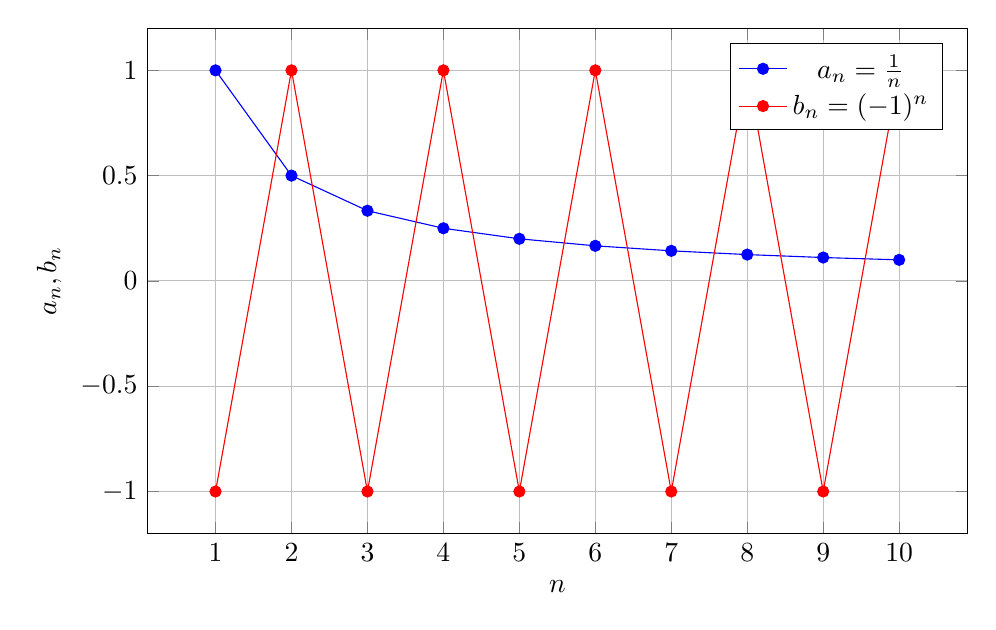
\begin{tikzpicture}
        \begin{axis}[
                xlabel={$n$},
                ylabel={$a_n, b_n$},
                legend pos=north east,
                grid=major,
                width=12cm,
                height=8cm,
            ]
            \addplot[
                domain=1:10,
                samples=10,
                mark=*,
                color=blue,
            ]
            {1/x};
            \addlegendentry{$a_n = \frac{1}{n}$}

            \addplot[
                domain=1:10,
                samples=10,
                mark=*,
                color=red,
            ]
            {(-1)^x};
            \addlegendentry{$b_n = (-1)^n$}
        \end{axis}
    \end{tikzpicture}
\end{center}
\begin{definition}
    We say that a sequence \((a_n)\) is \underline{convergent} if it converges for some \(L \in \mathbb{R}\). i.e.
    \[\exists L \in \mathbb{R}, \forall \epsilon > 0, \exists N \in \mathbb{N}, \forall n \geqslant N, \mid a_n - L \mid < \epsilon\]
\end{definition}\

\begin{definition}
    If \(a_n \rightarrow L\), then \(L\) is a \underline{limit} of \(a_n\).
\end{definition}

\begin{definition}
    A sequence \((a_n)\) is \underline{divergent} if it is not convergent, i.e.
    \[\forall L \in \mathbb{R}, \exists \epsilon > 0, \forall N \in \mathbb{N}\] such that \(|a_n - L| \geqslant \epsilon\)
\end{definition}

\begin{example}
    Let \(a_n = \frac{2^n - 1}{2^n}\). Then \(a_n \rightarrow 1\)
\end{example}
\begin{proof}
    Let \(\epsilon > 0\). Then \(|a_n - 1| = |\frac{2^n - 1}{2^n}| = |\frac{-1}{2^n}| = \frac{1}{2^n}\)
    We want to prove that \(\exists N \in \mathbb{N}\) such that \(\forall n \geqslant N, |a_n - 1| < \epsilon\)
    By Bernouli's Inequality, \(2^n = {(1 + 1)}^n.\)
    By Archimedean property, there exists \(N \in \mathbb{N}\) such that \(N > \frac{1}{\epsilon}\).
    \(\forall n \geqslant N, |a_n - 1| = \frac{1}{2^n} < \frac{1}{n} \leqslant \frac{1}{N} < \epsilon\). Hence, \(a_n \rightarrow 1\)
\end{proof}

Given \(a_n\) and \(L \in \mathbb{R}\), players A and B a game. \\

\begin{example}
    Let \[a_n = \frac{n^2 + n + 1}{3n^2 + 4}\]. Then \(a_n\) is convergent.
\end{example}
First we need to come up the limit of this sequence. \\
\[a_n = \frac{1 + \frac{1}{n} + \frac{1}{n^2}}{3 + \frac{4}{n^2}}\]
So \(\frac{1}{3}\) seems like a choice of limit \(L\).
\begin{proof}
    Let \(\epsilon > 0\). Then
    \begin{align*}
        \left| a_n - \frac{1}{3} \right|
    \end{align*}
    By the Archimedean property, \(\exists N \in \mathbb{N}\) such that \(\frac{1}{N} < \epsilon\). Hence for all, \(n \geqslant N\), \(\left| a_n - \frac{1}{3} \right| < \frac{1}{n} < \frac{1}{N} < \epsilon\)
\end{proof}

\begin{example}
    Let \[a_n = \frac{(-1)^n n^2 }{n^2 + 1}\]. Then \(a_n\) is divergent.
\end{example}
For large even \(n\), \[a_n = \frac{n^2}{n^2 + 1} = \frac{1}{1 + \frac{1}{n^2}}\]
For large odd \(n\), \[a_n = \frac{-n^2}{n^2 + 1} = -\frac{1}{1 + \frac{1}{n^2}}\]

\section{January 27, 2025}
\begin{theorem}[Limits respect Weak Inequalities]
    Let $(a_n)$ and $(b_n)$ be sequences such that $(a_n) \to L$ and $(b_n) \to M$. If $a_n \geq b_n$ for all $n$, then $L \geq M$.
\end{theorem}

\begin{proof}
    Suppose, for a contradiction, that $L < M$. Set $\epsilon = \frac{M - L}{2} > 0$. Since $a_n \to L$, there exists $N_1$ such that $n \geq N_1 \implies |a_n - L| < \epsilon$. Similarly, since $b_n \to M$, there exists $N_2$ such that $n \geq N_2 \implies |b_n - M| < \epsilon$. Therefore, for $n \geq \max(N_1, N_2)$, we have:
    \[
        a_n < L + \epsilon = \frac{L + M}{2} \quad \text{and} \quad b_n > M - \epsilon = \frac{L + M}{2}
    \]
    Hence, for $n \geq \max(N_1, N_2)$, we have $a_n < \frac{L + M}{2} < b_n$,
    which contradicts $a_n \geq b_n$ for all $n$.
\end{proof}

\begin{remark}
    Clearly, $\lim$ does not respect strict inequalities: e.g. $\frac{1}{n} > 0$ for all $n \geq 1$ but $0 = \lim \frac{1}{n} > \lim 0 = 0$ is false.
\end{remark}

\begin{theorem}[Squeeze Theorem]
    Suppose that $x_n \leq a_n \leq y_n$ for all $n$ and that $L = \lim x_n = \lim y_n$. Then $a_n \to L$ as $n \to \infty$.
\end{theorem}

\begin{proof}
    Let $\epsilon > 0$. Then there exist $N_1$ and $N_2$ such that $x_n - L > -\epsilon$ for all $n \geq N_1$, and $y_n - L < \epsilon$ for all $n \geq N_2$. So for $n \geq \max(N_1, N_2)$, we have:
    \[
        -\epsilon < x_n - L \leq a_n - L \leq y_n - L < \epsilon
    \]
    which shows that $a_n \to L$ also.
\end{proof}

\subsection{The Algebra of Limits}
Most sequences can be built up from simpler ones using addition,
multiplication, etc. The algebra of limits tells us how the corresponding
limits behave. Throughout the following, $(a_n)$ and $(b_n)$ denote sequences.

\begin{proposition}[AOL: Constants]
    If $a_n = a$ for all $n$, then $a_n \to a$.
\end{proposition}

\begin{proof}
    For any $\epsilon > 0$, take $N = 1$; $n \geq N \implies |a_n - a| = 0 < \epsilon$.
\end{proof}

\begin{proposition}[AOL: Sums]
    If $a_n \to a$ and $b_n \to b$, then $a_n + b_n \to a + b$.
\end{proposition}

\begin{proof}
    Let $\epsilon > 0$. Then $\frac{\epsilon}{2} > 0$ and so:
    \[
        \exists N_1 : n \geq N_1 \implies |a_n - a| < \frac{\epsilon}{2}, \quad \exists N_2 : n \geq N_2 \implies |b_n - b| < \frac{\epsilon}{2}
    \]
    Put $N_3 = \max(N_1, N_2)$. Then for all $n \geq N_3$, we have:
    \[
        |(a_n + b_n) - (a + b)| \leq |a_n - a| + |b_n - b| < \frac{\epsilon}{2} + \frac{\epsilon}{2} = \epsilon
    \]
\end{proof}

\begin{proposition}[AOL: Scalar Products]
    If $a_n \to a$ as $n \to \infty$ and $\lambda \in \mathbb{R}$, then $\lambda a_n \to \lambda a$.
\end{proposition}

\begin{proof}
    Let $\epsilon > 0$. Then $\frac{\epsilon}{|\lambda| + 1} > 0$ and so there exists $N$ such that $|a_n - a| < \frac{\epsilon}{|\lambda| + 1}$ for all $n \geq N$. Hence:
    \[
        |\lambda a_n - \lambda a| = |\lambda| |a_n - a| \leq \frac{|\lambda| \epsilon}{|\lambda| + 1} < \epsilon
    \]
    for all $n \geq N$.
\end{proof}

\begin{corollary}[AOL: Differences]
    If $a_n \to a$ and $b_n \to b$, then $a_n - b_n \to a - b$.
\end{corollary}

\begin{corollary}[AOL: Translations]
    If $a_n \to a$ and $c \in \mathbb{R}$, then $a_n + c \to a + c$.
\end{corollary}

\begin{lemma}
    If $x_n \to 0$ and $y_n \to 0$, then $x_n y_n \to 0$.
\end{lemma}

\begin{proof}
    Given $\epsilon > 0$, let $\epsilon_1 = \min(1, \epsilon) > 0$. Then:
    \[
        \exists N_1 : n \geq N_1 \implies |x_n| < \epsilon_1, \quad \exists N_2 : n \geq N_2 \implies |y_n| < \epsilon_1
    \]
    So if $n \geq \max(N_1, N_2)$, we have:
    \[
        |x_n y_n| \leq |x_n| |y_n| < \epsilon_1^2 \leq \epsilon
    \]
    which completes the proof.
\end{proof}

\begin{proposition}[AOL: Products]
    If $a_n \to a$ and $b_n \to b$, then $a_n b_n \to ab$.
\end{proposition}

\begin{proof}
    Note that:
    \[
        a_n b_n - ab = (a_n - a)(b_n - b) + b(a_n - a) + a(b_n - b)
    \]
    By the previous lemma, $(a_n - a)(b_n - b) \to 0$, and by Proposition 2.2.3,
    $b(a_n - a) \to 0$ and $a(b_n - b) \to 0$. Hence $a_n b_n \to ab$ by
    Proposition 2.2.2.
\end{proof}
\section{January 29, 2025}
\begin{proposition}[AOL: Reciprocals]
    If $a_n \to a$ and $a_n \neq 0$ for all $n$ and $a \neq 0$, then $\frac{1}{a_n} \to \frac{1}{a}$.
\end{proposition}

\begin{proof}
    Let $\epsilon > 0$. As $a \neq 0$ then $\frac{|a|}{2} > 0$. So there exists $N_1$ such that for $n \geq N_1$ we have $|a_n - a| < \frac{|a|}{2}$. By the Triangle Inequality
    \[
        |a| \leq |a_n| + |a - a_n| = |a_n| + |a_n - a|
    \]
    and so $|a_n| > \frac{|a|}{2}$ and $\left|\frac{1}{a_n}\right| <
        \frac{2}{|a|}$. Further, as $\frac{|a| \epsilon}{2} > 0$ then there exists
    $N_2$ such that for $n \geq N_2$
    \[
        |a_n - a| < \frac{|a| \epsilon}{2}.
    \]
    Set $N_3 = \max(N_1, N_2)$ so that for $n \geq N_3$
    \[
        \left|\frac{1}{a_n} - \frac{1}{a}\right| = \frac{|a_n - a|}{|a_n| |a|} < \frac{\frac{|a| \epsilon}{2}}{\frac{|a|}{2} |a|} = \epsilon.
    \]
\end{proof}

\begin{corollary}[AOL: Quotients]
    If $a_n \to a$, $b_n \to b$, and $b_n \neq 0$ for all $n$ and $b \neq 0$, then $\frac{a_n}{b_n} \to \frac{a}{b}$.
\end{corollary}

\begin{proposition}[AOL: Modulus]
    If $a_n \to a$ then $|a_n| \to |a|$.
\end{proposition}

\begin{proof}
    Exercise.
\end{proof}

\begin{example}
    $a_n = \frac{n^2 + n + 1}{3n^2 + 4} \to \frac{1}{3}$
\end{example}

\begin{proof}
    We write
    \[
        \frac{n^2 + n + 1}{3n^2 + 4} = \frac{1 + \frac{1}{n} + \frac{1}{n^2}}{3 + \frac{4}{n^2}} \to \frac{1 + 0 + 0}{3 + 0} = \frac{1}{3}
    \]
    noting
    \begin{itemize}
        \item $\frac{1}{n} \to 0$ by the Archimedean Property;
        \item $\frac{1}{n^2} \to 0$ by Proposition 2.2.7;
        \item $1 \to 1$;
        \item $1 + \frac{1}{n} + \frac{1}{n^2} \to 1$ by Proposition 2.2.2;
        \item $3 + \frac{4}{n^2} \to 3$ by Proposition 2.2.2;
        \item $\frac{1}{3 + \frac{4}{n^2}} \to \frac{1}{3}$ by Corollary 2.2.9;
        \item $a_n \to \frac{1}{3}$ by Proposition 2.2.7.
    \end{itemize}
\end{proof}

\begin{example}
    Suppose $a_1 = 1$, $a_2 = 1$, and we recursively define $a_{n+2} = a_{n+1} + a_n$, for $n \geq 1$.
\end{example}

\begin{proposition}
    $(\frac{a_{n+1}}{a_n})$ is convergent.
\end{proposition}

\begin{proof}
    By induction, $a_n \geq 1$ for all $n$. So for $n \geq 1$
    \[
        \frac{a_{n+2}}{a_{n+1}} = 1 + \frac{a_{n+1}}{a_n}.
    \]

    Write \(x_n = \frac{a_{n+1}}{a_n}\) for \(n \geq 1\). Note that \(x_n > 0\) for
    all \(n\). Then \(x_1 = 1\) and \(x_{n+1} = 1 + \frac{1}{x_n}\). Suppose that
    we did have convergence and that \(x_n \to x\). Since \(x_{n+1}\) is a tail of
    \(x_n\), we see that \((x_{n+1}) \to x$ and so $1 + \frac{1}{x_n} \to 1 +
    \frac{1}{x}$ by AOL. So
    \[
        x = 1 + \frac{1}{x}
    \]
    by the Uniqueness of Limits. Hence $x^2 - x - 1 = 0$ giving $x = \frac{1 \pm
            \sqrt{5}}{2}$. But $x_n \geq 0$ for all $n$, and so $x \geq 0$ by Theorem
    2.1.10 giving
    \[
        x = \frac{1 + \sqrt{5}}{2} > 1.
    \]
    At this point we don't yet know the sequence is convergent. We only know that
    if the sequence converges, then it must converge to the real number $\frac{1 +
            \sqrt{5}}{2}$, which we will denote $\phi$. Now we will show that $(x_n)$ does
    indeed converge to $\phi$. $\phi$ is called the Golden Ratio.
    \[
        x_{n+1} - \phi = 1 + \frac{1}{x_n} - \phi = 1 + \frac{1}{x_n} - 1 - \frac{1}{\phi} = \frac{1}{x_n} - \frac{1}{\phi} = \frac{x_n - \phi}{x_n \phi}
    \]
    as $\phi^2 = \phi + 1$. So
    \[
        \frac{x_{n+1} - \phi}{x_n - \phi} = \frac{1}{|x_n| |\phi|} = \frac{1}{\phi x_n} \leq \frac{1}{\phi}
    \]
    as $x_n \geq 1$ for all $n$. By induction, we get
    \[
        -\frac{1}{\phi^n} \leq x_n - \phi \leq \frac{1}{\phi^n}.
    \]
    and are done by the Squeeze Theorem, since $\phi > 1$ and so $(\pm
        \frac{1}{\phi^n}) \to 0$.
\end{proof}
\section{January 31, 2025}
\section{February 3, 2025}
\begin{example}\label{2.3.2}
    Let $a_n = n$ and $b_n = (2n + 1)^2$. Then $(a_n)$ and $(b_n)$ are strictly increasing.
\end{example}

\begin{definition}\label{2.3.3}
    We say that a sequence $(a_n)$ is:
    \begin{enumerate}
        \item bounded above if the set $S = \{a_n \mid n \in \mathbb{N}\}$ is bounded above.
        \item bounded below if the set $S = \{a_n \mid n \in \mathbb{N}\}$ is bounded below.
        \item bounded if the set $S = \{a_n \mid n \in \mathbb{N}\}$ is bounded.
    \end{enumerate}
\end{definition}

\begin{theorem}[Monotone Convergence Theorem] \label{2.3.4}
    The power of this theorem is that we can show a sequence converges without first calculating its limit.
    \begin{enumerate}
        \item Let $(a_n)$ be an increasing, bounded above sequence. Then $(a_n)$ converges.
        \item Let $(a_n)$ be a decreasing, bounded below sequence. Then $(a_n)$ converges.
    \end{enumerate}
\end{theorem}

\begin{proof}
    If $(a_n)$ is decreasing and bounded below, then $(-a_n)$ is increasing and bounded above, so it suffices to prove (1). We thus assume $(a_n)$ is increasing and bounded above.
    Let $L = \sup \{a_n \mid n \in \mathbb{N}\}$; this exists by the completeness axiom as the set is bounded above and non-empty. Let $\epsilon > 0$. By the Approximation Property there exists $N \in \mathbb{N}$ such that
    \[
        L - \epsilon < a_N \leq L.
    \]
    As the sequence is increasing, then for any $n \geq N$
    \[
        L - \epsilon < a_N \leq a_n \leq L,
    \]
    which implies $\forall n \geq N \mid a_n - L \mid < \epsilon$. That is $(a_n)
        \to L$.
\end{proof}

\begin{corollary}\label{2.3.5}
    Let $(a_n)$ be a bounded monotone sequence. Then $(a_n)$ converges.
\end{corollary}

\begin{example}\label{2.3.6}
    Let $x > 0$. Set $a_1 = 1$ and $a_{n+1} = \frac{1}{2} \left( a_n + \frac{x}{a_n} \right)$ for each $n$. Then $(a_n)$ converges to some positive number $a$ such that $a^2 = x$.
\end{example}

\begin{proof}
    By induction, it follows that $a_n$ is defined and $a_n > 0$ for all $n \geq 1$. We remark that for all $n$, we have $2a_n a_{n+1} = a_n^2 + x$. Therefore,
    \[
        0 \leq (a_n - a_{n+1})^2 = a_n^2 - 2a_n a_{n+1} + a_{n+1}^2 = a_{n+1}^2 - x,
    \]
    and so $a_{n+1}^2 \geq x$ for all $n \geq 1$. We now show that $(a_{n+1})$ is
    decreasing. Indeed, for $n \geq 2$,
    \[
        a_n - a_{n+1} = a_n - \frac{1}{2} \left( a_n + \frac{x}{a_n} \right) = \frac{a_n^2 - x}{2a_n} \geq 0.
    \]
    Therefore, $a_n \geq a_{n+1}$ for all $n \geq 2$. Therefore the sequence
    $(a_{n+1})$ is decreasing and bounded below by $0$, hence converges to some $a
        \geq 0$. Since $a_{n+1}^2 \geq x$ for all $n \geq 1$, AOL implies $a^2 \geq x >
        0$, and so $a > 0$. Moreover, since $(a_{n+1})$ is a tail of $(a_n)$, it
    follows that $(a_n)$ also converges to $a$. Since $a_{n+1} = \frac{1}{2} \left(
        a + \frac{x}{a} \right)$, $a > 0$ and $a > 0$, AOL implies that
    \[
        a = \frac{1}{2} \left( a + \frac{x}{a} \right).
    \]
    Rearranging gives $x = a^2$, as required.
\end{proof}

\subsection{Subsequences}

\begin{example}\label{2.4.1}
    Let $a_n = \frac{1}{n^2}$, i.e.
    \[
        (a_n) = \left( 1, \frac{1}{4}, \frac{1}{9}, \frac{1}{16}, \frac{1}{25}, \ldots \right).
    \]
    We can get new sequences by looking at:
    \begin{itemize}
        \item everything after the second place $\left( \frac{1}{9}, \frac{1}{16},
                  \frac{1}{25}, \ldots \right)$
        \item all odd terms $\left( 1, \frac{1}{9}, \frac{1}{25}, \ldots \right)$
        \item all prime terms $\left( \frac{1}{4}, \frac{1}{9}, \frac{1}{25}, \ldots \right)$
    \end{itemize}
\end{example}

\begin{definition}\label{2.4.2}
    Let $(a_n)$ be a sequence. We say that a sequence $(b_n)$ is a subsequence of $(a_n)$ if there is a strictly increasing sequence of natural numbers $(f(n))$ such that $(b_n) = (a_{f(n)})$. (There may be more than one such function $f$.) Often we write $n_r$ for $f(r)$ and write a subsequence as $(a_{n_r})$ or $(a_{n_r})_{r=1}^\infty$.
\end{definition}

\begin{example}\label{2.4.3}
    Let
    \[
        (a_n) = \left( n^2 \right) = (1, 4, 9, 16, \ldots)
    \]
    \[
        (b_n) = (0) = (0, 0, 0, 0, \ldots)
    \]
    \[
        (f(n)) = (2n) = (2, 4, 6, 8, \ldots)
    \]
    \[
        (g(n)) = (2n - 1) = (1, 3, 5, 7, \ldots)
    \]
    Then
    \[
        (a_{f(n)}) = (a_{2n}) = (4, 16, 36, 64, \ldots)
    \]
    \[
        (a_{g(n)}) = (a_{2n+1}) = (1, 9, 25, 49, \ldots)
    \]
    \[
        (b_{f(n)}) = (b_{2n}) = (0, 0, 0, 0, \ldots)
    \]
    \[
        (b_{g(n)}) = (b_{2n+1}) = (0, 0, 0, 0, \ldots)
    \]
\end{example}

\begin{proposition}\label{2.4.4}
    Suppose that the sequence $(a_n)$ converges to $L$. Then every subsequence $(a_{n_r})$ also converges to $L$.
\end{proposition}

\begin{proof}
    Let $\epsilon > 0$. Then there exists $N$ such that
    \[
        n \geq N \implies |a_n - L| < \epsilon.
    \]
    As $r \mapsto n_r$ is increasing then $n_r \geq r$ for all $r$ and so
    \[
        r \geq N \implies n_r \geq N \implies |a_{n_r} - L| < \epsilon.
    \]
\end{proof}
\section{February 5, 2025}
\begin{theorem}[Monotone Subsequence Theorem]\label{2.4.5}
    Let \((a_n)\) be a sequencce. Then \((a_n)\) has a monotone subsequence which means the subsequence is either increaing or decreasing over that bound.
\end{theorem}
\begin{definition}[Vantage Point]

\end{definition}
\begin{center}
    \begin{tikzpicture}
        \draw[->] (0,0) -- (10,0) node[right] {$n$};
        \draw[->] (0,0) -- (0,5) node[above] {$a_n$};

        \foreach \x in {1,2,...,9}
        \draw (\x,0.1) -- (\x,-0.1) node[below] {\x};

        \foreach \y in {1,2,...,4}
        \draw (0.1,\y) -- (-0.1,\y) node[left] {\y};

        \draw[thick, color=blue] plot coordinates {(1,1) (2,3) (3,2) (4,4) (5,3.5) (6,4.5) (7,3.8) (8,4.2) (9,4.6)};

        \node at (4,4) [circle,fill,inner sep=1.5pt,label=above:$a_k$] {};
        \draw[dashed] (4,4) -- (4,0);
        \draw[dashed] (4,4) -- (0,4);

        \node at (6,4.5) [circle,fill,inner sep=1.5pt,label=above:$a_m$] {};
        \draw[dashed] (9,4.6) -- (0,4.6);

        \node at (2,3) [circle,fill,inner sep=1.5pt,label=above:$a_j$] {};
        \draw[dashed] (2,3) -- (0,3);
    \end{tikzpicture}
\end{center}

Here, \(a_k\), \(a_m\), and \(a_j\) are vantage points.

\begin{proof}
    We say that \(k \in \mathbb{N}\) is a `vantage point' of \((a_n)\) if \(a_m < a_k\) for all \(m > k\). Let \(V = \{k \in \mathbb{N} \mid k \text{ is a vantage point}\}\).
    \begin{itemize}
        \item \textbf{Case 1: \(V\) is infinite:} \\ Let \(V = \{k_1, k_2, \ldots \}\) where \(k_1 < k_2 < k_3 < \ldots\). Each \(k_i\) is a vantage point. If \(m > n\), then \(a_{{k_m}} < a_{k_n}\). Hence \((a_{k_n})_{n=1}^\infty\) is a decreasing subsequence.
        \item \textbf{Case 1: \(V\) is finite:} \\ There exist \(k_1\) such that \(\forall n \geq k_1, a_n\) is not a vantage point, \(\exists k_2 > k_1\) such that \(k_2 > k_1)\) Since, \(k_2 > k_1\) is also not a vantage point. hence \(\exists k_3 > k_2\) such that \(a_{k_3} \geq a_{k_2}\).\\ We continue in this way, defining a strictly increaseing subsequence. \[k_1 < k_2 < k_3 < \ldots\] such that \[a_{k_1} \leq a_{k_2} \leq a_{k_2} \leq a_{k_3} \leq \ldots\]. Hence \((a_{k_n})_{n=1}^\infty\) is an increasing subsequence. Therefore, \((a_{k_n})_{n=1}^\infty\) is monotone.    

    \end{itemize}
\end{proof}

\begin{theorem}[Bolzano-Weierstrass Theorem]\label{2.4.6}
Let \((a_n)\) be a bouded sequence. Then \((a_n)\) has a convergent-subsequence.
\end{theorem}
\begin{proof}
    By \cref{2.4.5}, \((a_n)\) has a monotone subsequence, \((a_{k_n})_{n=1}^\infty\). Since \((a_n)\) is bounded, so is \((a_{k_n})\). By the Montone Convergence Theorem, \((a_{k_n})\) is convergent.
\end{proof}
\begin{proof}
    Let $(a_n)$ be a bounded sequence. Then there exist $A_1$ and $B_1$ such that $A_1 \leq a_n \leq B_1$ for all $n$. We construct a nested sequence of intervals $[A_n, B_n]$ as follows: Let $[A_2, B_2]$ be one of the intervals $[A_1, \frac{A_1 + B_1}{2}]$ or $[\frac{A_1 + B_1}{2}, B_1]$ such that $\{n \in \mathbb{N} \mid a_n \in [A_2, B_2]\}$ is infinite. Similarly, let $[A_3, B_3]$ be one of the intervals $[A_2, \frac{A_2 + B_2}{2}]$ or $[\frac{A_2 + B_2}{2}, B_2]$ such that $\{n \in \mathbb{N} \mid a_n \in [A_3, B_3]\}$ is infinite. We continue this process, ensuring that each interval $[A_n, B_n]$ contains infinitely many terms of the sequence $(a_n)$. We then pick a subsequence $k_1 < k_2 < \ldots < k_n$ such that $a_{k_n} \in [A_n, B_n]$. Since $B_n - A_n = \frac{B_1 - A_1}{2^{n-1}}$, the length of the intervals $[A_n, B_n]$ tends to $0$ as $n \to \infty$. Since $(A_n)$ and $(B_n)$ are monotone and bounded, they converge to the same limit $L$. By the Squeeze Theorem, the subsequence $(a_{k_n})$ converges to $L$.
\end{proof}
%\section{February 10, 2025}
%\section{February 12, 2025}
%\section{February 14, 2025}
%\section{February 17, 2025}
%\section{February 19, 2025}
%\section{February 21, 2025}
%\section{February 24, 2025}
%\section{February 26, 2025}
%\section{February 28, 2025}
%\section{March 3, 2025}
%\section{March 5, 2025}
%\section{March 7, 2025}
%\section{March 17, 2025}
%\section{March 19, 2025}
%\section{March 21, 2025}
%\section{March 24, 2025}
%\section{March 26, 2025}
%\section{March 28, 2025}
%\section{March 31, 2025}
%\section{April 2, 2025}
%\section{April 4, 2025}
%\section{April 7, 2025}
%\section{April 9, 2025}
%\section{April 11, 2025}
%\section{April 14, 2025}
%\section{April 16, 2025}
%\section{April 18, 2025}
%\section{April 21, 2025}
%\section{April 23, 2025}
%\section{April 25, 2025}
%\section{April 28, 2025}
%\section{April 30, 2025}
%%%%%%%%%%%%%%%%%%%%%%%
\end{document}